\documentclass[tikz,border=8pt]{standalone}
\usepackage{tikz}
\usepackage{pgfplots}
\usepackage{amsmath,amssymb}
\usepackage[T1]{fontenc}
\usepackage{lmodern}
\usepackage{xcolor}
\usetikzlibrary{arrows.meta,positioning,shapes.geometric,fit,calc,backgrounds,matrix}
\pgfplotsset{compat=1.18}
\definecolor{ink}{HTML}{18202A}
\definecolor{blue}{HTML}{2563EB}
\definecolor{bluefill}{HTML}{EAF1FF}
\definecolor{green}{HTML}{14804A}
\definecolor{greenfill}{HTML}{E8F6EE}
\definecolor{amber}{HTML}{B56A00}
\definecolor{amberfill}{HTML}{FFF3D6}
\definecolor{red}{HTML}{B42318}
\definecolor{redfill}{HTML}{FDECEC}
\definecolor{gray}{HTML}{667085}
\definecolor{light}{HTML}{F4F6F8}
\definecolor{linegray}{HTML}{C7CDD4}
\tikzset{
  box/.style={draw=ink, rounded corners=3pt, very thick, fill=white, align=center, inner sep=7pt, font=\sffamily\small},
  bluebox/.style={box, fill=bluefill, draw=blue},
  greenbox/.style={box, fill=greenfill, draw=green},
  amberbox/.style={box, fill=amberfill, draw=amber},
  redbox/.style={box, fill=redfill, draw=red},
  ghost/.style={draw=linegray, rounded corners=3pt, thick, fill=light, align=center, inner sep=7pt, font=\sffamily\small},
  label/.style={font=\sffamily\footnotesize, text=gray, align=center},
  title/.style={font=\sffamily\bfseries\large, text=ink, align=center},
  arrow/.style={-{Latex[length=3mm,width=2mm]}, very thick, draw=ink},
  bluearrow/.style={-{Latex[length=3mm,width=2mm]}, very thick, draw=blue},
  redarrow/.style={-{Latex[length=3mm,width=2mm]}, very thick, draw=red},
  greenarrow/.style={-{Latex[length=3mm,width=2mm]}, very thick, draw=green}
}

\begin{document}
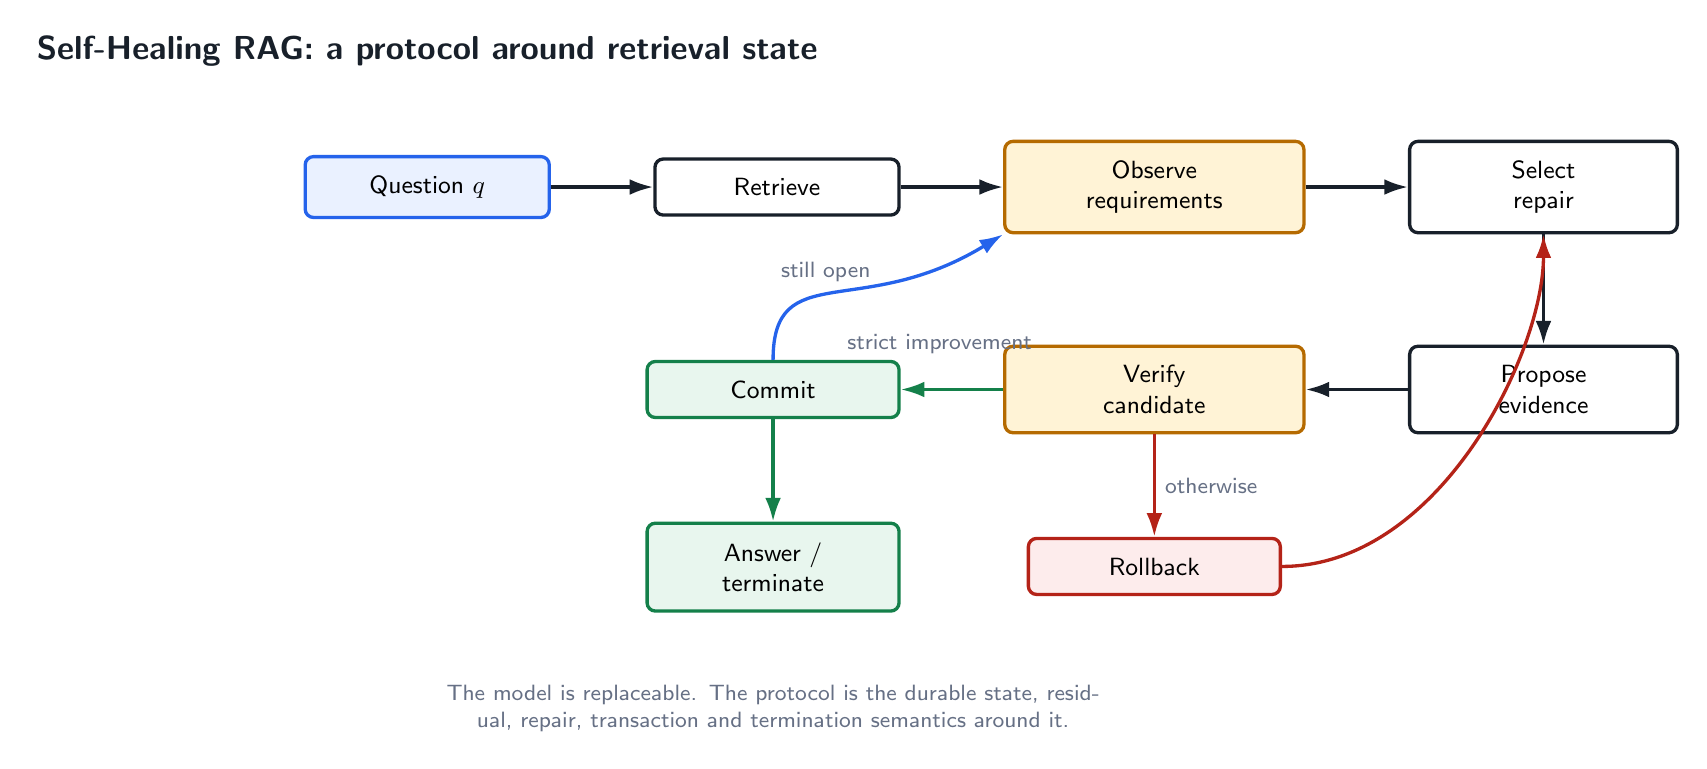
\begin{tikzpicture}[node distance=11mm and 13mm]
\node[title] (ttl) {Self-Healing RAG: a protocol around retrieval state};
\node[bluebox, below=10mm of ttl, minimum width=31mm] (q) {Question $q$};
\node[box, right=of q, minimum width=31mm] (ret) {Retrieve};
\node[amberbox, right=of ret, minimum width=38mm] (obs) {Observe\\requirements};
\node[box, right=of obs, minimum width=34mm] (act) {Select\\repair};
\node[box, below=14mm of act, minimum width=34mm] (prop) {Propose\\evidence};
\node[amberbox, left=of prop, minimum width=38mm] (verify) {Verify\\candidate};
\node[greenbox, left=of verify, minimum width=32mm] (commit) {Commit};
\node[redbox, below=13mm of verify, minimum width=32mm] (rollback) {Rollback};
\node[greenbox, below=13mm of commit, minimum width=32mm] (answer) {Answer /\\terminate};
\draw[arrow] (q)--(ret);
\draw[arrow] (ret)--(obs);
\draw[arrow] (obs)--(act);
\draw[arrow] (act)--(prop);
\draw[arrow] (prop)--(verify);
\draw[greenarrow] (verify)--node[label,above=9pt,pos=.62]{strict improvement}(commit);
\draw[redarrow] (verify)--node[label,right]{otherwise}(rollback);
\draw[greenarrow] (commit)--(answer);
\draw[bluearrow] (commit.north) .. controls +(0,13mm) and +(-18mm,-11mm) .. node[label,above,pos=.46]{still open}(obs.south west);
\draw[redarrow] (rollback.east) .. controls +(20mm,0) and +(0,-15mm) .. (act.south);
\node[label, below=8mm of answer, text width=130mm] {The model is replaceable. The protocol is the durable state, residual, repair, transaction and termination semantics around it.};
\end{tikzpicture}
\end{document}
